\documentclass{article}
\usepackage[margin=1in,a4paper]{geometry}
\usepackage[utf8]{inputenc}
\usepackage{hyperref}
\usepackage{amsmath}
\usepackage{gensymb}
\usepackage{enumitem,amssymb}
\newlist{checks}{itemize}{2}
\setlist[checks]{label=$\square$}
\usepackage{graphicx}
\usepackage{amsthm}
\usepackage{amsfonts}
\usepackage{pdfpages}
\usepackage{pgfplots}
\pgfplotsset{compat=newest}
\usetikzlibrary{calc}
\usepackage{mathtools}
\usepackage{array}
\usepackage[T1]{fontenc}
\usepackage{lmodern}
\usepackage{tabularx}
\usepackage{fancyhdr}

\usepackage{xcolor}
\usepackage{nicefrac}
\usepackage{mdframed}
\usepackage[boxed,vlined]{algorithm2e}
\usepackage{cleveref}
% \usepackage{graphicx}
\newcommand{\Lim}[1]{\raisebox{0.0ex}{\scalebox{1}{$\displaystyle \lim_{#1}\;$}}}
\usepackage{graphicx}
\usepackage{tkz-tab}
\usepackage{fdsymbol}

\newcommand{\R}{\mathbb{R}}
\newcommand{\C}{\mathbb{C}}
\newcommand{\w}{\omega}
\newcommand{\p}{\partial}
\newcommand{\si}{&\quad\text{si }}
\DeclareMathOperator{\sinc}{sinc}
\DeclareMathOperator{\interior}{int}
\DeclareMathOperator{\adh}{adh}
\DeclareMathOperator{\argcosh}{argcosh}
\DeclareMathOperator{\argsinh}{argsinh}

\newtheorem{example}{Exemple}

\title{Corrigé des exercices - Analyse}
\author{Team Analyse}
\date{Septembre 2021}

\begin{document}

\maketitle

\section{Limites, suites et fonctions}
\subsection{Exercice 1 ($\medblackstar \medwhitestar \medwhitestar$)}

Les relations 1, 2, 3, 4 et 6 sont des fonctions, mais pas les relations 5 et 7 car pour ces deux relations certains $x$ ont pour image plusieurs $y$. Les plus perspicaces diront que les domaines de définition et d'arrivée n'ont pas été définis pour la première relation, et qu'ainsi $h$ ne serait pas une fonction, ce qui ne serait strictement pas faux. Cependant, en analyse, vous définirez implicitement les fonctions sur le plus grand ensemble de définition possible, avec $\R$ comme domaine d'arrivée.

\subsection{Exercice 2 ($\medblackstar \medwhitestar \medwhitestar$)}

\begin{enumerate}
    \item On a :
    \begin{gather*}
        \Lim{n \to + \infty} \frac{n^2 + 2}{7} = +\infty\\
        \Lim{n \to + \infty} \frac{3}{n} = 0
    \end{gather*}
    Selon la règle d'addition des limites, $+\infty + 0 = +\infty$\\
    Donc $\Lim{n \to + \infty} \frac{n^2 + 2}{7} + \frac{3}{n} = +\infty$\\
    \item $$a_n = \frac{7n^4 + 2}{4n^4} = \frac{7 + \frac{2}{n^4}}{4}$$
    On a $\Lim{n \to + \infty} \frac{2}{n^4} = 0$\\
    Donc $\Lim{n \to + \infty} a_n = \Lim{n \to + \infty} \frac{7 + \frac{2}{n^4}}{4} = \frac{7}{4}$\\
    \item $$a_n = \frac{5n^2 + 2n + 1}{n^3 + 5} = \frac{\frac{5}{n} + \frac{2}{n^2} + \frac{1}{n^3}}{1 + \frac{5}{n^3}}$$
    On a $\Lim{n \to + \infty} \frac{5}{n} = \Lim{n \to + \infty} \frac{5}{n^3} = \Lim{n \to + \infty} \frac{2}{n^2} = \Lim{n \to + \infty} \frac{1}{n^3} = 0$\\
    Selon la règle de division des limites, $\frac{0}{1} = 0$\\
    Donc $\Lim{n \to + \infty} a_n = \frac{\frac{5}{n} + \frac{2}{n^2} + \frac{1}{n^3}}{1 + \frac{5}{n^3}} = 0$\\
\end{enumerate}

\subsection{Exercice 3 ($\medblackstar \medblackstar \medwhitestar$)}

Trouver les limites des suites suivantes si elles existent lorsque $n$ tend vers $+\infty$ :

\begin{enumerate}
    \item On a : $$\Lim{n \to + \infty} \frac{6}{n} = 0 \quad \mbox{ et } \quad \Lim{n \to + \infty} \cos(2 n) \mbox{ n'existe pas}$$
    Si on additionne une suite qui converge avec une suite qui diverge, la somme diverge forcément.\\
    Donc $(a_n)$ diverge.
    \item Étant donné que $\cos$ est périodique de période $2\pi$, on a : $$\Lim{n \to + \infty} \frac{6}{n} = 0 \quad \mbox{ et } \quad \Lim{n \to + \infty} \cos(2\pi n) = 1$$
    Selon la règle d'addition des limites, $a_n$ converge vers 1.
    \item On résout cette limite avec le théorème des deux gendarmes.
    Pour tout $n \in \mathbb{N}$ :
    $$0 \leq n \leq e^n$$
    Donc on a :
    $$\frac{\ln(e^n + 0)}{n} \leq \frac{\ln(e^n + n)}{n} \leq \frac{\ln(e^n + e^n)}{n}$$
    En simplifiant les deux suites aux extrimités on obtient :
    $$1 \leq \frac{\ln(e^n + n)}{n} \leq \frac{\ln(e^n + e^n)}{n} =\frac{\ln(2e^n)}{n}= \frac{\ln(2) + \ln(e^n)}{n} = \frac{\ln(2) + n}{n}$$
    On remarque que les deux suites aux extrémités convergent vers 1, donc $a_n$ converge vers 1 également.
    \item On résout cette limite en multipliant pas le complémentaire :
    \begin{align*}
        \sqrt{n^2 + 4} - \sqrt{n^2 +n - 3} &= \frac{(\sqrt{n^2 + 4} - \sqrt{n^2 +n - 3})(\sqrt{n^2 + 4} + \sqrt{n^2 +n - 3})}{\sqrt{n^2 + 4} + \sqrt{n^2 +n - 3}}\\
        &= \frac{n^2 + 4 - n^2 - n + 3}{\sqrt{n^2 + 4} + \sqrt{n^2 +n - 3}}\\
        &= \frac{- n + 7}{\sqrt{n^2 + 4} + \sqrt{n^2 +n - 3}}\\
        &= \frac{- n + 7}{n\sqrt{1 + \frac{4}{n^2}} + n\sqrt{1 + \frac{1}{n} - \frac{3}{n^2}}}\\
        &= \frac{- 1 + \frac{7}{n}}{\sqrt{1 + \frac{4}{n^2}} + \sqrt{1 + \frac{1}{n} - \frac{3}{n^2}}}
    \end{align*}
    On a $\Lim{n \to + \infty} \frac{7}{n} = \Lim{n \to + \infty} \frac{4}{n^2} = \Lim{n \to + \infty} \frac{1}{n} = \Lim{n \to + \infty} \frac{3}{n^2} = 0$\\
    Donc $\Lim{n \to + \infty} a_n = -\frac{1}{2}$
\end{enumerate}

\subsection{Exercice 4 ($\medblackstar \medblackstar \medwhitestar$)}

\begin{enumerate}
    \item Il y a beaucoup de $\ln(x)$ non ? Voyons-y plus clair en posant $y = \ln(x)$. Ainsi, la limite à étudier devient $\Lim{y \to 0^+} y\ln(y)$ puisque $\Lim{x \to 1^+} \ln(x) = 0^+$, et en $0^+$ $y\ln(y)$ tend vers $0$.
    $$
    \Lim{y \to 0^+} y\ln(y) \overset{t = \frac{1}{y}}{=}\Lim{t \to +\infty} \frac{\ln\left(\frac{1}{t}\right)}{t} = \Lim{t \to +\infty} \frac{-\ln(t)}{t} \overset{u = ln(t)}{=} \Lim{u \to +\infty} -\frac{u}{e^u} = 0
    $$
    \item Rappelez-vous : $\sin(t) = \sin(\pi-t)$. Ainsi, $\sin(2x) = \sin(\pi-2x)$. On obtient donc :
    $$
    \Lim{x \to \frac{\pi}{2}} \frac{\sin(\pi-2x)}{\pi -2x} \overset{y = \pi-2x}{=} \Lim{y \to 0} \frac{\sin(y)}{y} = 1
    $$
\end{enumerate}

\subsection{Exercice 5 ($\medblackstar \medblackstar \medwhitestar$)}

\begin{itemize}
    \item $b_n = \cos(2\pi n)$ converge (vers 1) mais $a_n = 2\pi n$ diverge.
    \item $b_n = \lvert {(-1)}^n \rvert$ converge (vers 1) mais $a_n = {(-1)}^n$ diverge.
    \item En prenant $b_n = 0$ et $a_n = (-1)^{n+1}$ pour tout $n \in \mathbb{N}$, les suites satisfont les conditions, $(b_n)$ converge (vers 0), mais $(a_n)$ ne converge pas.
\end{itemize}

\subsection{Exercice 6 ($\medblackstar \medblackstar \medblackstar$)}

1) Définition de $\Lim{x \to a} f(x) = l$ :
\begin{center}
    Pour tout $\epsilon > 0$, il existe un $\delta_l >0$ tel que pour tout $x \in \mathbb{R}$ : $0 < \lvert x - a \rvert \leq \delta_l$, on a $\lvert f(x) - l \rvert \leq \epsilon$
\end{center}
Définition de $\Lim{x \to a} f(x) = m$ :
\begin{center}
    Pour tout $\epsilon > 0$, il existe un $\delta_m >0$ tel que pour tout $x \in \mathbb{R}$ : $0 < \lvert x - a \rvert \leq \delta_m$, on a $\lvert f(x) - m \rvert \leq \epsilon$
\end{center}
\noindent 2) $\delta = \min(\delta_l, \delta_m)$\\

\noindent 3) Réarrangeons d'abord le 4 : $$\epsilon = \frac{\lvert l - m \rvert}{4} \iff 4\epsilon = \lvert l - m \rvert$$
Il suffit de faire ensuite apparaître le terme $f(x)$ :
$$4\pi = \lvert l - m \rvert = \lvert l - f(x) + f(x) - m \rvert$$
Puis on applique l'inégalité du triangle :\\
$$4\epsilon = \lvert l - f(x) + f(x) - m \rvert \leq \lvert l - f(x) \rvert + \lvert f(x) - m \rvert $$
\noindent 4) D'après les deux définitions du 1) et le 2) pour tout $\epsilon$, donc en particulier quand $\epsilon = \frac{\lvert l - m \rvert}{4}$, il existe un $\delta$ tel que pour tout $x \in \mathbb{R}$ : $0 < \lvert x - a \rvert \leq \delta$, on a $\lvert f(x) - l \rvert \leq \epsilon$ et $\lvert f(x) - m \rvert \leq \epsilon$.\\
En considérant que $x$ soit à une distance $\delta$ de $a$ dans notre inéquation du 3), on a donc $$4\epsilon \leq \lvert f(x) - l \rvert + \lvert f(x) - m \rvert \leq \epsilon + \epsilon = 2\epsilon$$
En conséquent :
$$4\epsilon \leq 2\epsilon \iff 4\epsilon - 2\epsilon \leq 0 \iff 2 \epsilon \leq 0 \iff \epsilon \leq 0$$
Ce qui est une contradiction du postulat de base !

\section{Continuité}

\subsection{Exercice 1}
\noindent $g$ est continue sur $\mathbb{R}\setminus\{-1,0,1\}$. \newline
Etudions sa continuité en ces $3$ points en posant $X = \ln(|x|)$: \newline
-En $0$, on a $\displaystyle\lim_{x \to 0} g(x)=\lim_{X \to -\infty} \frac{1}{X}=0=g(0)$ \newline
-En $1$, on a $\displaystyle\lim_{x \to 1^{+}} g(x)=\lim_{X \to 0^{+}} \frac{1}{X}=+\infty$ \newline
En procédant de même avec $-1$, on trouve finalement que $g$ est continue en $0$ mais pas en $-1$ et $1$.

\subsection{Exercice 2}
\noindent Soit $g(x)=f(x)-x$. $g(x)$ est à valeurs dans $[-1,1]$ et est continue comme différence de fonction continue. Il existe au moins une valeur $x_1$ telle que $g(x_1) \leq 0$, en effet: $\forall x \in \ [0;1] \ f(x) \leq 1 \iff f(x) - 1 \leq 0 \implies g(1) = f(1) - 1 \leq 0 \implies x_1 = 1$. De même, il existe au moins une valeur $x_2$ telle que $g(x_2) \geq 0$, en effet: $\forall x \in \ [0;1] \ f(x) \geq 0 \iff f(x) - 0 \geq 0 \implies g(0) = f(0) - 0 \geq 0 \implies x_2 = 0$. Alors, par corollaire du TVI, $\exists x_3 \in [0;1]$ tel que $g(x_3) = f(x_3) - x_3 = 0 \iff f(x_3) = x_3$. Cela conclut la preuve.
\subsection{Exercice 3}
\noindent En partant de $\sin(x) < x < \tan(x)$ pour tout $x$ tel que $0 < x < \frac{\pi}{2}$, on obtient :
\begin{gather*}
    \sin(x) < x < \tan(x)\\
    \frac{\sin(x)}{\sin(x)} < \frac{x}{\sin(x)} < \frac{\tan(x)}{\sin(x)}\\
    1 < \frac{x}{\sin(x)} < \frac{1}{\cos(x)}\cdot\frac{\sin(x)}{\sin(x)}\\
    1 < \frac{x}{\sin(x)} < \frac{1}{\cos(x)}
\end{gather*}
On remarque que $\frac{1}{\cos(x)}$ tend vers 1 lorsque $x$ tend vers 0 (car $\Lim{x \to 0} \cos(x) = 1$)
D'après le théorème des deux gendarmes, $\frac{x}{\sin(x)}$ tend aussi vers 1 lorsque $x$ tend vers 0.
Nous avons donc : 
$$\Lim{x \to 0}\frac{\sin(x)}{x} = \frac{1}{\Lim{x \to 0}\frac{x}{\sin(x)}} = \frac{1}{1} = 1$$
\subsection{Exercice 4}
\noindent De $f(x)^{2}=1$ on déduit que $f(x)=\pm 1$ pour tout $x\in \mathbb{R}$.\newline
Reste à prouver que $f$ ne peut atteindre qu'une seule de ces deux valeurs. Par l'absurde supposons qu'il existe $x_{1},x_{2}$ tq $f(x_{1})=1$ et $f(x_{2})=-1$. Comme $f$ est continue alors par TVI il existe un point $x_3$ en lequel $f(x_3)=0$ (ou n'importe quel autre valeur dans $]-1,1[$), mais ainsi $f(x_3)^2 = 0 = 1$, absurde.\\
Remarque : les deux propositions suivantes sont \textit{très} différentes :
\begin{enumerate}
    \item $\forall x \in \R$, $f(x) = 1$ ou $f(x) = -1$.
    \item $\forall x \in \R f(x) = 1$ ou $\forall x \in \R f(x) = - 1$.
\end{enumerate}
Dans le premier cas (qui est une partie de l'hypothèse dans cet exercice), chaque $x$, indépendamment des autres, peut avoir $1$ ou $-1$ pour image. Dans le second cas, ce sont soit tous les $x$ à la fois qui ont pour image $1$, soit tous les $x$ à la fois qui ont pour image $-1$.
\section{Séries}
\subsection{Exercice 1}
\begin{enumerate}
    \item La somme des $n$ premiers entiers est une formule qui mérite d'être retenue. Ici, on reconnaît une suite $(a_n)$ arithmétique de raison 1, définie par récurrence~:
    \[
    \begin{cases}
    a_0 & = 0 \\
    a_{n+1} & = a_{n} + 1
    \end{cases}
    \]
    Comme vu durant le cours, la somme des termes d'une suite arithmétique de $k = 1$ à $k = n$ est égale à~:
    \[
    \sum_{k = 1}^{n} a_n = \underbrace{n}_{\textrm{nb. de termes}}\cdot \overbrace{\frac{a_1 + a_n}{2}}^{\textrm{moyenne des extrêmes}}
    \]
    Ainsi, la somme des $n$ premiers entiers est égale à~:
    \[
    \boxed{
    \sum_{k = 1}^{n} k = \sum_{k = 1}^{n} a_k = \frac{n(n+1)}{2}
    }
    \]
    La somme des $100$ premiers entiers est donc égale à $\frac{100\cdot 101}{2} = 5050$.
    
    \item Cette somme est une série géométrique de raison $\frac{1}{2}$, on applique simplement la formule, \emph{en n'oubliant pas que $k$ commence à $1$ et donc qu'il faut soustraire le premier terme}~:
    \[
    \boxed{
    \sum_{k = 1}^{100} \left ( \frac{1}{2} \right )^k = \frac{1- \left (\frac{1}{2} \right )^{101}}{1-\frac{1}{2}} \underbrace{- 1}_{\left ( \frac{1}{2}\right )^0} = 1 - \left ( \frac{1}{2} \right )^{100}
    }
    \]
    
    \item En utilisant le hint donné, on développe facilement~:
    \[
    \frac{1}{k(k+1)} = \frac{1}{k} - \frac{1}{k+1}
    \]
    Il est possible de généraliser, sans l'aide donnée, le procédé de décomposition de ce type de fractions rationnelles (i.e. les quotients de polynômes). On appelle cette méthode la \emph{décomposition en éléments simples}~: on laisse en annexe le détail de cette méthode. Il est important de la connaître puisqu'elle permettra de simplifier certaines sommes et (plus tard) des intégrales type examen, mais vous n'avez pas à la connaître dès maintenant.
    
    Pour la somme, on remarque que chaque terme s'annule, sauf le premier et le dernier. En effet, par changement d'indice, on obtient~:
    \[
    \sum_{k=1}^{100} \frac{1}{k(k+1)} = \sum_{k = 1}^{100} \left ( \frac{1}{k} - \frac{1}{k+1} \right ) = \left ( \sum_{k = 1}^{100} \frac{1}{k} \right ) - \left ( \sum_{k' = 2}^{101} \frac{1}{k'} \right )
    \]
    où $k' = k + 1$ est le changement d'indice (ainsi, si $1 \leq k \leq 100$ alors $2 \leq k' \leq 101$). Par abus de notation, on omet souvent de changer de lettre, et on garde $k$ pour les deux sommes, puisque leur contexte d'utilisation est différent. Les valeurs des indices 2 à 100 des 2 sommes se neutralisent, si bien qu'il ne reste que 2 termes~:
    \[
    \boxed{
    \sum_{k = 1}^{100} \frac{1}{k(k+1)} = 1 - \frac{1}{101} = \frac{100}{101}
    }
    \]
    Ce type de somme où les termes s'annulent de proche en proche est appelé une \emph{somme téléscopique}. Pour une telle somme de la forme $\displaystyle\sum_{k = 1}^{n} \left ( a_{k} - a_{k+1} \right )$, on a la formule~:
    \[
    \boxed{
    \sum_{k = 1}^{n} a_{k} - a_{k+1} = a_1 - a_{n+1}
    }
    \]
    
    \item Tout comme la somme précédente, on retrouve une \emph{somme téléscopique}, qui se simplifie drastiquement après un changement de variable~:
    \[
    \boxed{
    \sum_{k=2}^{100} \left( \frac{1}{\sqrt{k-1}} - \frac{1}{\sqrt{k}}\right ) = \left ( \sum_{k = 1}^{99} \frac{1}{\sqrt{k}}\right ) - \left (
    \sum_{k = 2}^{100} \frac{1}{\sqrt{k}} \right ) = 1 - \frac{1}{\sqrt{100}} = \frac{9}{10}
    }
    \]
\end{enumerate}

\subsection{Exercice 2}
On a vu en cours que l'utilité des séries absolument convergentes réside principalement dans le fait que la convergence absolue des séries est suffisante pour assurer la convergence normale. Cependant, l'implication inverse est \emph{fausse}, et c'est une erreur fréquente. En effet, on peut (grossièrement) comprendre qu'une série peut contenir des termes positifs et négatifs, ce qui leur permet tout de même de faire converger la série en s'annulant, mais la série des valeurs absolues peut être arbitrairement grande, et donc divergerait.

\noindent Plus formellement, un contre-exemple suffit à infirmer cette proposition. La \emph{série harmonique alternée}, introduite en cours, est généralement l'exemple de choix, puisque la série converge, avec~:
\[
\sum_{n = 1}^{\infty} \frac{(-1)^n}{n} = -\ln(2)
\]
Mais pourtant la série de valeur absolue est la \emph{série harmonique} $\displaystyle\sum_{n = 1}^{\infty} \frac{1}{n}$, qui diverge.

\subsection{Exercice 3}
\begin{enumerate}
    \item Il suffit de montrer le cas $n = 0$ et l'étape de récurrence~:
    \begin{itemize}
        \item \underline{Base :} Pour $n = 0$, l'égalité est vérifiée puisque
        \[
        \sum_{k = 0}^{0} x^k = x^0 = 1 \quad \textrm{ et } \quad \frac{1 - x^1}{1 - x} = 1
        \]
        \item \underline{Induction :} Supposons que 
        \[
        \sum_{k = 0}^{n} x^k = \frac{1 - x^{n+1}}{1-x}
        \]
        Alors on a~:
        \[
        \sum_{k = 0}^{n+1} x^k = \sum_{k = 0}^{n} x^k + x^{n+1} \overset{(*)}{=} \frac{1 - x^{n+1}}{1-x} + x^{n+1}
        \]
        où l'on a utilisé en $(*)$ l'hypothèse de récurrence. Ainsi, l'équation se réduit à~:
        \[
        \frac{1-x^{n+1} + (1-x)x^{n+1}}{1-x} = \frac{1 - x^{n+2}}{1-x}
        \]
        Ce qui est bien ce que l'on cherche. Donc l'égalité est vraie pour tout $n \in \mathbb{N}$.
    \end{itemize}
    
    \item Par définition des séries numériques, on obtient grâce au point ci-dessus~:
    \[
    \sum_{k = 0}^{\infty} x^k = \lim_{n \to \infty} \sum_{k = 0}^{n} x^k = \begin{cases}
    \displaystyle\lim_{n \to \infty} \frac{1 - x^{n+1}}{1-x} & \textrm{si } x \neq 1 \\
    \displaystyle\lim_{n \to \infty} n + 1 & \textrm{si } x = 1
    \end{cases}
    \]
    On distingue alors 4 cas~:
    \begin{itemize}
        \item Si $x = 1$ alors la série diverge trivialement puisque $\displaystyle\lim_{n \to \infty} n + 1 = \infty$.
        \item Si $x = -1$ alors la série diverge de même puisque $\displaystyle\lim_{n \to \infty} (-1)^{n+1}$ n'existe pas.
        \item Si $|x| > 1$ alors $\displaystyle\lim_{n \to \infty} x^{n+1}$ est infinie si $x > 0$ ou n'existe pas si $x < 0$. Ainsi \emph{la série diverge}.
        \item Si $|x| < 1$ alors $\displaystyle\lim_{n \to \infty} x^{n+1} = 0$, et donc la série converge~:
        \[
        \boxed{
        \sum_{k = 0}^{\infty} x^k = \frac{1}{1-x}
        }
        \]
    \end{itemize}
    Le domaine de convergence de la série est donc l'ensemble $D = \left ] -1, 1 \right [$.
\end{enumerate}

\subsection{Exercice 4}
\textit{Rappel :} Les critères de convergence qui suivent sont tous basés sur l'étude des \emph{séries de Riemann}, c'est-à-dire les séries de la forme
\[
\sum_{n = 1}^{\infty} \frac{1}{n^s}
\]
qui convergent si et seulement si $s > 1$. En particulier la série harmonique $\displaystyle\sum_{n = 1}^{\infty} \frac{1}{n}$ diverge.

\begin{enumerate}
    \item Pour tout $n > 0$, on a l'inéquation suivante~:
    \[
    \sqrt[3]{n} \leq n \implies \frac{1}{\sqrt[3]{n}} \geq \frac{1}{n} \implies \sum_{n = 1}^{\infty} \frac{1}{\sqrt[3]{n}} \geq \sum_{n = 1}^{\infty} \frac{1}{n}
    \]
    Puisque la série harmonique diverge, par critère de comparaison la série diverge. On aurait pu remarquer plus directement que $\sqrt[3]{n} = n^{\frac{1}{3}}$ et donc la série est une série de Riemann de paramètre $s = \frac{1}{3} < 1$, ce qui implique qu'elle diverge.
    
    \item Premièrement, on simplifie le terme général pour pouvoir appliquer le critère de comparaison~:
    \[
    \frac{n(n-1)}{n^{\frac{8}{3}}} = \frac{n - 1}{n^{\frac{5}{3}}} \overset{n \geq 2}{\geq} \frac{\frac{1}{2}n}{n^{\frac{5}{3}}} = \frac{1}{2} \frac{1}{n^{\frac{2}{3}}}
    \]
    En effet $n - 1 \geq \frac{1}{2}n$ si et seulement si $\frac{1}{2}n \geq 1$, i.e. $n \geq 2$. Ainsi par le critère de comparaison, puisque $\displaystyle \sum_{n = 1}^{\infty} \frac{1}{n^{\frac{2}{3}}}$ est une série de Riemann divergente, la série diverge.
    
    Une autre méthode consiste à considérer que le terme général de la série est équivalent à~:
    \[
    \frac{n(n - 1)}{n^{\frac{8}{3}}} \sim \frac{n^2}{n^{\frac{8}{3}}} = \frac{1}{n^{\frac{2}{3}}}
    \]
    où l'on note $(a_n) \sim (b_n)$ si on a $\displaystyle\lim_{k \to \infty} \frac{a_k}{b_k} = 1$ (on dit que les deux suites sont \emph{équivalentes} à l'infini). Ainsi la série $\displaystyle\sum_{n = 1}^{\infty} \frac{n(n-1)}{n^{\frac{8}{3}}}$ est de même nature (c'est-à-dire converge ou diverge en même temps) que la série $\displaystyle\sum_{n = 1}^{\infty} \frac{1}{n^{\frac{2}{3}}}$ qui diverge. Cette méthode, qui s'appelle le critère d'équivalence, marche uniquement \emph{lorsque les 2 séries sont de termes positifs}. Ce type de raisonnement par ordre de grandeur a l'avantage d'être plus rapide, car il permet d'estimer rapidement la convergence d'une série en la comparant à une série similaire connue -- généralement les séries de Riemann. Il se retrouvera notamment plus tard dans les calculs de complexité en AICC I.
    
    \item En se rappelant du graphe du logarithme naturel, on sait que pour tout $n \geq 2$~:
    \[
    \log(n) \geq 1 \implies n^2\log(n) \geq n^2 \implies \frac{1}{n^2\log(n)} \leq \frac{1}{n^2}
    \]
    On a donc la comparaison de série suivante~:
    \[
    \sum_{n = 2}^{\infty} \frac{1}{n^2\log(n)} \leq \sum_{n = 2}^{\infty} \frac{1}{n^2}
    \]
    où la série à droite \emph{converge} (on a d'ailleurs $\displaystyle\sum_{n = 1}^{\infty} \frac{1}{n^2} = \frac{\pi^2}{6}$, résultat établi par Euler en 1741). Ainsi la série à gauche converge de même par le critère de comparaison.
    
    \item Il suffit pour cette série de minorer $(-1)^n$, de telle sorte qu'on obtient~:
    \[
    a + (-1)^n \geq a - 1 \implies \sum_{n = 1}^{\infty} \frac{a + (-1)^n}{n} \geq \sum_{n = 1}^{\infty} \frac{a - 1}{n} = (a - 1) \sum_{n = 1}^{\infty} \frac{1}{n}
    \]
    où la série de droite est $a - 1$ fois la série harmonique divergente. Donc la série diverge pour tout $a > 1$.
\end{enumerate}

\subsection{Exercice 5}
\begin{enumerate}
    \item Il suffit d'utiliser la définition des séries numériques ainsi que la linéarité de la limite~:
    \begin{align*}
    \sum_{n = 0}^{\infty} (a_n + b_n) & = \lim_{N \to \infty} \sum_{n = 0}^{N} (a_n + b_n) \\
    & = \lim_{N \to \infty} \left ( \sum_{n = 0}^{N} a_n \right ) + \left ( \sum_{n = 0}^{N} b_n \right ) \\
    & = \left ( \lim_{N \to \infty} \sum_{n = 0}^{N} a_n \right ) + \left ( \lim_{N \to \infty} \sum_{n = 0}^{N} b_n \right ) \\
    & = \underbrace{\sum_{n = 0}^{\infty} a_n}_{\in\ \mathbb{R}} + \underbrace{\sum_{n = 0}^{\infty} b_n}_{\in\ \mathbb{R}} \in \mathbb{R}
    \end{align*}
    où on a pu utiliser dans la 3ème ligne la linéarité de la limite puisque les deux limites existent et sont finies.
    
    \item Par la définition de la suite $(a_n^+)$, on a~:
    \[
    a_n^+ = \begin{cases}
    a_n + |a_n| = 2|a_n| & \textrm{si } a_n \geq 0 \\
    a_n - a_n = 0    & \textrm{si } a_n < 0
    \end{cases}
    \]
    On en déduit que pour tout $n \in \mathbb{N}$, on a l'encadrement $0 \leq a_n^+ \leq 2 |a_n|$ et donc~:
    \[
    0 \leq \sum_{n = 0}^{\infty} a_n^+ \leq 2 \sum_{n = 0}^{\infty} |a_n| = 2l \in \mathbb{R}
    \]
    Puisque $\displaystyle\sum_{n = 0}^{\infty} a_n^+$ est une série de termes positifs et majorée (par $2l$), elle converge.
    
    \item Remarquons d'abord que $a_n = a_n + |a_n| - |a_n| = a_n^+ - |a_n|$ et donc la série de terme général $a_n$ s'exprime comme
    \[
    \sum_{n = 0}^{\infty} a_n = \sum_{n = 0}^{\infty} \left ( a_n^+ - |a_n| \right )
    \]
    Puisque les séries $\displaystyle\sum_{n = 0}^{\infty} a_n^+$ et $\displaystyle\sum_{n = 0}^{\infty} |a_n|$ sont convergentes (par 2. et par hypothèse, respectivement), on en déduit par 1. que la série $\displaystyle\sum_{n = 0}^{\infty} a_n$ converge comme somme de séries convergentes.
\end{enumerate}

\section{Nombres complexes}

\subsection{Exercice 1}
\begin{itemize}
    \item z = $\sqrt{3}-i$. Conformément à la définition de partie réelle et imaginaire, on à $Re(z) = \sqrt{3}$ et $Im(z) = -1$. Le module est quant à lui donné par $|z| = \sqrt{{Re(z)}^2+{Im(z)}^2} = \sqrt{\sqrt{3}^2+(-1)^2}= 2$. Comme $Re(z)>0$, en suivant la formule du cours, on trouve $arg(z) =\arctan{ \frac{Im(z)}{Re(z)}} = \arctan{\frac{1}{\sqrt{3}}} = \frac{\pi}{6} $  \\
    On peut donc exprimer $z$ sous la forme polaire de la façon suivante : $z = 2(\cos{\frac{\pi}{6}}+i\sin{\frac{\pi}{6}})$ \\
    Ainsi que sous la forme exponentielle : $z = 2e^{i\frac{\pi}{6} }$
    \item $z = -4$. On a cette fois $Re(z)=-4$ et pas de partie imaginaire (elle est nulle), c'est à dire que $z$ est un nombre réel. Pour calculer $|z|$ et $arg(z)$, on pourrait utiliser les formules, mais on préfère ici utiliser "l'intuition" du plan complexe. Pour rappel, les nombres complexes peuvent être placés dans un plan, ou l'axe des abscisses dénote la partie réelle, et l'axe des ordonnées, la partie imaginaire. Si on relie par un trait le nombre complexe considéré à l'origine du plan, la longueur de ce trait correspond en fait au module, et l'angle entre ce dernier et l'axe réel positif, à l'argument. Ici, $z$ est un réel, on le place donc sur l'axe réel. Ainsi l'angle ne peut être que de 0, si $z > 0$ ou de $\pi$ si $z < 0$.
\begin{center}
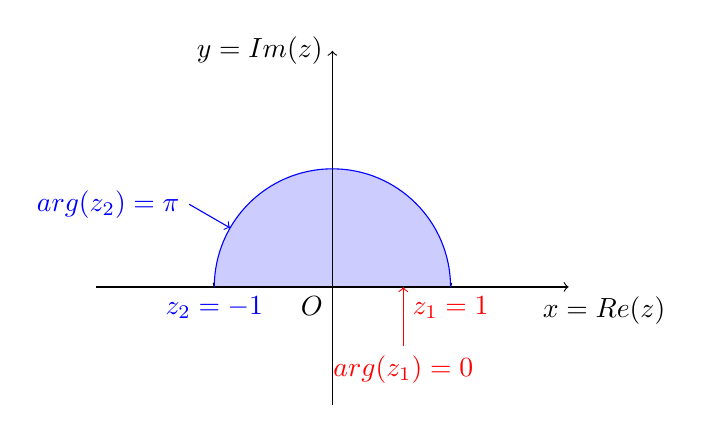
\begin{tikzpicture}[scale = 1.5]
\fill [color = blue!20] (0:1) arc (0:180:1);
\draw [->] (0,0) -- (90:2);
\draw [->] (0,0) -- (0:2);
\draw (0,0) -- (180:2);
\draw (0,0) -- (-90:1);
\draw (0:1)--(2:1.01);
\draw (180:1)--(178:1.01);
\draw  (0:1) node[below,red]{$z_1 = 1$};
\draw  (180:1) node[below,blue]{$z_2 = -1$};
\draw [blue] (0:1) arc (0:180:1);
\draw  (150:1.4) node[left,blue]{$arg(z_2)=\pi$};
\draw [->,blue] (150:1.4) -- (150:1);
\draw  (0.6,-0.5) node[below,red]{$arg(z_1)=0$};
\draw [->,red] (0.6,-0.5) -- (0:0.6);
\draw  (0,0) node[below left]{$O$};
\draw  (0:2.3) node[below]{$x = Re(z)$};
\draw  (90:2) node[left]{$y = Im(z)$};
\end{tikzpicture} 
\end{center}
Pour $z = -4$, on trouve alors $arg(z) = \pi$ et $|z| = 4$ sans procéder au moindre calcul ! La forme polaire et exponentielle de $z$ sont alors respectivement données par : $z = 4(\cos{\pi}+i\sin{\pi})$ et $z = 4e^{i\pi}$
\item $z = 8i$. On a cette fois $Im(z) = 8$ et pas de partie réelle, c'est à dire que $z$ est un imaginaire pur. On utilisera encore le plan complexe pour déduire sans calcul le module et l'argument de $z$. En effet, comme le montre l'image suivante, un imaginaire pur ne peut avoir en argument seulement $\pm \frac{\pi}{2}$, selon le signe de $Im(z)$. 

\begin{center}
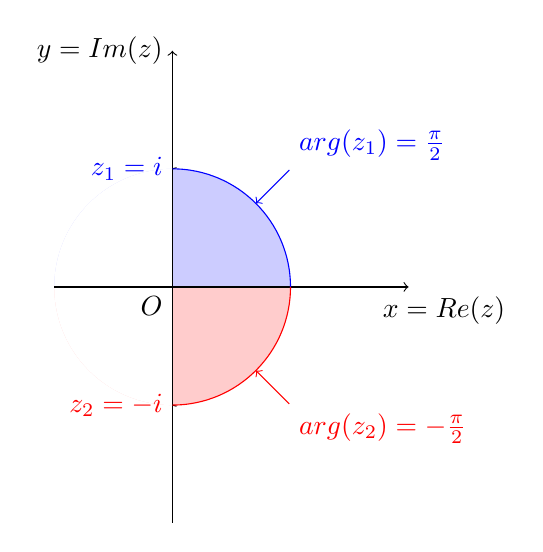
\begin{tikzpicture}[scale = 1.5]
\fill [color = blue!20] (0:1) arc (0:180:1);
\fill [color = red!20] (0:1) arc (0:-180:1);
\fill [color = white!100] (0,1) arc (90:270:1);
\draw [->] (0,0) -- (90:2);
\draw [->] (0,0) -- (0:2);
\draw (0,0) -- (180:1);
\draw (0,0) -- (-90:2);
\draw (90:1)--(88:1.01);
\draw (-90:1)--(-88:1.01);
\draw  (90:1) node[left,blue]{$z_1 = i$};
\draw  (-90:1) node[left,red]{$z_2 = -i$};
\draw  (45:1.4) node[above right,blue]{$arg(z_1)=\frac{\pi}{2}$};
\draw [->,blue] (45:1.4) -- (45:1);
\draw  (-45:1.4) node[below right,red]{$arg(z_2)=-\frac{\pi}{2}$};
\draw [->,red] (-45:1.4) -- (-45:1);
\draw  (0,0) node[below left]{$O$};
\draw  (0:2.3) node[below]{$x = Re(z)$};
\draw  (90:2) node[left]{$y = Im(z)$};
\draw [blue] (0:1) arc (0:90:1);
\draw [red] (0:1) arc (0:-90:1);
\end{tikzpicture} 
\end{center}
Comme $Im(z)>0$ on trouve sans calculer que $|z|= 8$ et $arg(z)=\frac{\pi}{2}$. La forme polaire et exponentielle de $z$ sont alors respectivement données par : $z = 8(\cos{\frac{\pi}{2}}+i\sin{\frac{\pi}{2}})$ et $z = 8e^{i\frac{\pi}{2}}$
\item $z = \dfrac{1-i}{i}$. Ici, il semble à priori difficile de dégager une partie imaginaire/réelle à cause de la fraction. Pour se ramener à une forme plus commode, on souhaite transformer le dénominateur en un réel, et pour cela, on va le multiplier par $i$. On a alors : $z = \dfrac{1-i}{i}= \dfrac{i\times(1-i)}{i\times i} = -(i+1)$. Sous cette forme, il est bien plus facile de traiter le problème et on trouve $Re(z) = Im(z) = -1$. On pourrait encore trouver l'argument en utilisant le plan complexe, mais c'est moins évident, et on préfère le faire par le calcul ce qui donne $arg(z) = \arctan {1}+\pi = \frac{\pi}{4} + \pi = \dfrac{5\pi}{4} \left( \overset{\mod 2\pi}{=} -\frac{3\pi}{4} \right)$. On a ici ajouté $\pi$ étant donné que $Re(z) < 0$ (voir la formule donnée dans les slides). Le module est quant à lui donné par $|z| = \sqrt{(-1)^2+(-1)^2} = \sqrt{2}$. La forme polaire et exponentielle de $z$ sont alors respectivement données par : $z = \sqrt{2}(\cos{\frac{3\pi}{4}}+i\sin{\frac{3\pi}{4}})$ et $z = \sqrt{2}e^{i\frac{3\pi}{4}}$

\end{itemize}

\subsection{Exercice 2}
1) On sait que par définition $\cos{\theta}+i\sin{\theta} = e^{i\theta}$. Cela correspond en fait aux formes polaires et exponentielles d'un nombre complexe de module 1 et d'argument $\theta$. A partir de ça, on trouve : 
\begin{equation*}
    (\cos{\theta}+i\sin{\theta})^n=(e^{i\theta})^n=e^{in\theta}=\cos{n\theta}+i\sin{n\theta}
\end{equation*}
2) La formule de Moivre appliquée pour $n = 2$ donne : 
\begin{equation*}
    \cos{2\theta}+i\sin{2\theta} = (\cos{\theta}+i\sin{\theta})^2 = \cos^2{\theta}+2i\sin{\theta}\cos{\theta}-\sin^2{\theta}
\end{equation*}
En faisant correspondre les termes réels et imaginaires des deux expressions, on trouve :
\begin{equation*}
\begin{cases}
    \cos{2\theta} = \cos^2{\theta}-\sin^2{\theta}\\ \sin{2\theta}=2\sin{\theta}\cos{\theta}
\end{cases}
\end{equation*}
3)\begin{itemize}
    \item En suivant la définition de conjugué on trouve : 
    \begin{itemize}
        \item $z = 9+4i \Rightarrow \bar z = 9-4i$
        \item $z = i  \Rightarrow \bar z = -i = -z $. Le conjugué d'un imaginaire pur $z$ est toujours donné par $-z$.
        \item $z = 4  \Rightarrow \bar z = 4 = z $. Le conjugué d'un réel $z$ est toujours égal à lui même.
    \end{itemize}
    \item $z\bar z = (x +iy)(x-iy)=x^2-(iy)^2=x^2+y^2=|z|^2 $
    \item En observant le conjugué dans le plan complexe ,on s'aperçoit que $\bar z$ est juste le symétrique de $z$ par rapport à l'axe réel. Ainsi leur distance à l'origine (le module) est la même, et leur angle sont opposés. On a donc $|z| = |\bar z|$ et $arg(z) = -arg(\bar z)$. 

\begin{center}
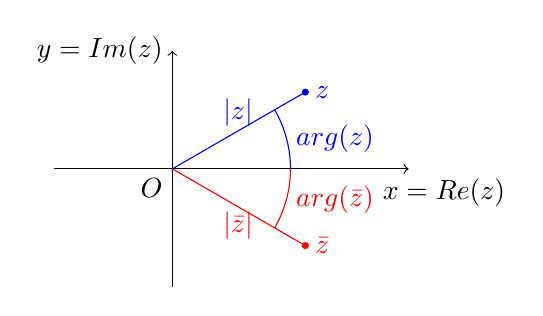
\begin{tikzpicture}[scale = 1.5]
%\fill [color = blue!20] (0:1) arc (0:180:1);
\draw [->] (0,0) -- (90:1);
\draw [->] (0,0) -- (0:2);
\draw (0,0) -- (180:1);
\draw (0,0) -- (-90:1);
\fill [blue] (30:1.3) circle (0.03);
\fill [red] (-30:1.3) circle (0.03);
\draw [blue] (30:1.3) node[right]{$z$};
\draw [blue] (32:0.9) node[left]{$|z|$};
\draw [blue] (15:1) node[right]{$arg(z)$};
\draw [red] (-15:1) node[right]{$arg(\bar z)$};
\draw [red] (-30:1.3) node[right]{$\bar z$};
\draw [red] (-32:0.9) node[left]{$|\bar z|$};
\draw [blue] (0,0) -- (30:1.3);
\draw [red] (0,0) -- (-30:1.3);
\draw  (0,0) node[below left]{$O$};
\draw  (0:2.3) node[below]{$x = Re(z)$};
\draw  (90:1) node[left]{$y = Im(z)$};
\draw [blue] (30:1) arc (30:0:1) ;
\draw [red] (-30:1) arc (-30:0:1) ;
\end{tikzpicture} 
\end{center}
\end{itemize}
La démonstration de ces identités serait facile, mais on voulait ici vous faire travailler votre intuition du plan complexe. \\

\noindent 4) Pour déterminer les parties réelles et imaginaires des différents complexes, on essaiera à chaque fois de les ramener sous la forme $z = x +iy$ :
\begin{itemize}
    \item $z = \dfrac{1-i}{3+i}$. Lorsqu'un complexe est présenté sous la forme d'une fraction de deux complexes, il existe une méthode pour ramener à tous les coups le dénominateur sous forme réel. Si on pose $z_2$ le dénominateur, il suffit en fait de le multiplier par son conjugué pour le 'transformer' en réel, puisque comme on l'a vu avant $z\bar z = |z|^2$, qui est un réel. Pour cet exemple on a donc : 
    \begin{equation*}
        z = \dfrac{1-i}{3+i} = \dfrac{3-i}{3-i}\dfrac{1-i}{3+i}=\dfrac{2-4i}{10}
    \end{equation*}
    On a donc $Re(z) = \frac{1}{5}$ et $Im(z) = -\frac{2}{5}$
    \item $z = (2-i)^8$. Ici le but est clairement pas de développer l'expression. On va plutôt développer $z_2 = 2-i$ sous forme polaire puis appliquer la formule de Moivre. On a $|z_2| = \sqrt{5}$ et $arg(z_2) = \arctan{(-\frac{1}{2})}$. Sous forme polaire, on a donc : $z_2=\sqrt{5}\left[\cos\left(\arctan\left(-\frac{1}{2}\right)\right)+i\sin\left(\arctan\left(-\frac{1}{2}\right)\right)\right]$.
    En utilisant la formule de Moivre, on obtient
    \begin{equation*}
        z = z_2^8=5^{\frac{8}{2}}\left[\cos\left(8\arctan\left(-\frac{1}{2}\right)\right)+i\sin\left(8\arctan{(-\frac{1}{2})}\right)\right]=625\left[\cos\left(8\arctan\left(-\frac{1}{2}\right)\right)+i\sin\left(8\arctan\left(-\frac{1}{2}\right)\right)\right]
    \end{equation*}
    On trouve alors $Re(z) = 625\cos(8\arctan{(-\frac{1}{2}}))$ et $Im(z) = 625\sin{(8\arctan{(-\frac{1}{2})}})$.
    \item $z= (\frac{1}{i})^{47}$. Ici, on refait pareil qu'a la question précédente, mais rassurez-vous, ce sera pas aussi fastidieux. On pose $z_2 = \frac{1}{i}=-i$, qui sous forme polaire s'écrit comme $z_2 = \cos{(-\frac{\pi}{2})}+i\sin{(-\frac{\pi}{2})}$. On a alors :
    \begin{equation*}
        z = z_2^{47}=\cos\left(-\frac{47\pi}{2}\right)+i\sin\left(-\frac{47\pi}{2}\right) = \cos\left(-\frac{\pi}{2}\right)+i\sin\left(-\frac{\pi}{2}\right)=-i
    \end{equation*}
    Donc $Im(z) = -1$.
\end{itemize}
\subsection{Exercice 3}
Vous avez appris avant de rejoindre l'EPFL que les racines d'un polynôme du second degré (réel) $ax^2+bx +c$ sont données par :
\begin{equation*}
    x_{1,2} = \dfrac{-b\pm\sqrt{b^2-4ac}}{2a}
\end{equation*}
Avec $x_1 = x_2$ lorsque $\Delta = b^2-4ac = 0$. Pour le même polynôme, mais à valeurs dans	$\mathbb{C}$, les racines sont données par les mêmes formules que précédemment, mais avec comme subtilité que lorsque $\Delta < 0$, on peut cette fois bien calculer des racines.  \\
Ici le polynôme est $z^2-2z+2$. En utilisant l'indication de l'énoncé, on a alors que les racines sont données par :
\begin{equation*}
    z_{1,2} = \dfrac{2\pm\sqrt{-4}}{2}=\dfrac{2\pm i\sqrt{4}}{2} = 1\pm i
\end{equation*}

\noindent L'équation $z^2-2z+2 = 0$ admet donc deux solutions données par $z_1= 1+i$ et $z_2 = 1-i$. 



\subsection{Exercice 4}

Il existe plusieurs manières d'aborder ce problème et on va en présenter deux ici. La première consiste à poser $z = x +iy$ et de résoudre un système. En effet dans ce cas là on a : 
\begin{equation*}
    z^2 = 1-i \iff x^2+2ixy-y^2 = 1-i
\end{equation*}
En faisant correspondre les coefficients réels et imaginaires, on trouve :
\begin{equation*}
    \begin{cases}
        x^2-y^2=1 \\
        2xy = -1
    \end{cases}
    \Rightarrow
     \begin{cases}
        x = \pm\sqrt{1+y^2} \\
        \pm\sqrt{1+y^2}y =-\frac{1}{2} 
    \end{cases}
\end{equation*}
Pour que les équations aient une solution, on voit ici qu'il faut que $x$ et $y$ soient de signes opposés. 
\begin{equation*}
    \begin{cases}
        x = \pm\sqrt{1+y^2} \\
        (1+y^2)y^2 =\frac{1}{4} 
    \end{cases} \\
    \Rightarrow
     \begin{cases}
        x = \pm\sqrt{1+y^2} \\
        y^4+y^2 -\frac{1}{4}=0 
    \end{cases} \\
\end{equation*}
On pose $Y = y^2$ et la dernière équation devient : $Y^2+Y-\frac{1}{4} = 0$.
Cette équation admet deux solutions, $Y_1 = \dfrac{-1-\sqrt{2}}{2}$ et $Y_2 = \dfrac{-1+\sqrt{2}}{2}$. Pour se ramener à l'équation initiale, on doit résoudre $y^2=Y_1$ et $y^2 = Y_2$. Comme $Y_1 < 0$, la première équation n'a pas de solution, tandis que la deuxième équation à deux solutions données par $y_{\pm}=\pm\sqrt{\frac{-1+\sqrt{2}}{2}}$. On rapelle ici que $y$ est réel, seul $z$ est complexe ! 

\noindent On trouve avec ça deux couples de solutions :
\begin{equation*}
    \begin{cases}
       y_+ = \sqrt{\frac{-1+\sqrt{2}}{2}} \\
       x_-  = -\sqrt{1+( \sqrt{\frac{-1+\sqrt{2}}{2}})^2} =  -\sqrt{\frac{1+\sqrt{2}}{2}}
    \end{cases}
    \quad \textrm{ainsi que } \quad
     \begin{cases}
       y_- = -\sqrt{\frac{-1+\sqrt{2}}{2}} \\
       x_+  = \sqrt{1+(- \sqrt{\frac{-1+\sqrt{2}}{2}})^2} =  \sqrt{\frac{1+\sqrt{2}}{2}}
    \end{cases}
\end{equation*}
Finalement l'équation $z^2 = 1-i$ admet deux solutions :
\begin{equation*}
    z_1 = -\sqrt{\frac{1+\sqrt{2}}{2}}+i \sqrt{\frac{-1+\sqrt{2}}{2}}
    \qquad
    \textrm{et}
    \qquad z_2 = \sqrt{\frac{1+\sqrt{2}}{2}}-i \sqrt{\frac{-1+\sqrt{2}}{2}}=-z_1
\end{equation*}

\noindent Une deuxième méthode consiterait à utiliser la formule de Moivre. En effet, par cette dernière on sait que $arg(z^n)+2k\pi = n \cdot arg(z)$. Ici $arg(z^2) = \arctan{(-1)} = -\frac{\pi}{4} \Rightarrow arg(z) = -\frac{\pi}{8}$ ou $arg(z) =  \frac{-\frac{\pi}{4}+2\pi}{2} = \frac{7\pi}{8}$. D'autre part, comme on a que $|z|^2 = |z^2|$, on trouve que $|z| = \sqrt{|z^2|} = \sqrt{\sqrt{2}}= 2^{\frac{1}{4}}$. Finalement on trouve logiquement que l'équation $z^2 = 1 -i$ a deux solutions, données par : 
\begin{equation*}
  \quad z_1 = 2^{\frac{1}{4}}\left[\cos\left(-\frac{\pi}{8}\right)+i\sin\left(-\frac{\pi}{8}\right)\right] \quad \textrm{et} \quad z_2= 2^{\frac{1}{4}}\left[\cos\left(\frac{7\pi}{8}\right)+i\sin\left(\frac{7\pi}{8}\right)\right]
\end{equation*}
Les solutions trouvées sont bien les mêmes selon les deux méthodes, mais juste exprimées différement ! A vous de voir quelle méthode vous préférez pour résoudre ce genre d'équation, moi j'ai clairement une favorite...

\subsection{Exercice 5}
Utilisons la seconde méthode de l'exercice précédent. 
$$\sqrt{3}-i=\overline{\sqrt{3}+i} = 2\overline{\left(\frac{\sqrt{3}}{2}+i\frac{1}{2}\right)} = 2\overline{\left(\cos\left(\frac{\pi}{6}\right) + i\sin\left(\frac{\pi}{6}\right)\right)} = 2e^{-i\frac{\pi}{6}}
$$
En utilisant la dernière slide des complexes: l'ensemble des solutions est alors $\left\{\sqrt[6]{2}e^{i\frac{2\pi k - \frac{\pi}{6}}{6}} \ | \ k = 0, \hdots, 5\right\}$.

\break

\appendix
\section{Décomposition en éléments simples}
La \emph{décomposition en éléments simples} permet d'exprimer les fractions rationnelles de la forme $\frac{P(x)}{Q(x)}$, avec $P, Q$ des polynômes, en sommes de fractions rationnelles plus simples, comportant au dénominateur des polynômes divisant $Q$. Elle est utilisée lorsque $\mathrm{deg}(P) < \mathrm{deg}(Q)$, c'est-à-dire que la puissance la plus haute se trouve au dénominateur, car dans le cas contraire une division polynomiale peut être effectuée (via des méthodes comme le schéma de Horner, par exemple).
La méthode se décompose en plusieurs étapes~:
\begin{enumerate}
    \item Premièrement, il faut trouver la décomposition du polynôme $Q$~: par le théorème fondamental de l'algèbre ce polynôme peut se décomposer en polynômes de degré 1 ou 2 irréductibles (c'est-à-dire de la forme $ax^2 + bx + c$ avec $b^2 < 4ac$). Généralement, cette étape n'est pas nécessaire puisque les polynômes seront donnés sous leur forme factorisée, ou la factorisation est simple à trouver.
    
    \item Deuxièmement, pour chaque polynôme dans cette décomposition, on applique 2 règles~:
    \begin{itemize}
        \item Si le polynôme est de degré 1 (c'est-à-dire de la forme $x - x_0$) et de multiplicité $n$ (i.e. apparaissant $n$ fois dans la décomposition), alors on écrit~:
        \[
        \frac{P(x)}{Q(x)} = \frac{a_1}{x-x_0} + \frac{a_2}{(x-x_0)^2} + \ldots + \frac{a_n}{(x-x_0)^n} + R(x)
        \]
        où $R(x)$ est le reste de la méthode sur les autres facteurs de $Q$.
        \item Si le polynôme est de degré 2 irréductible et de multiplicité $n$, alors similairement on écrit~:
        \[
        \frac{P(x)}{Q(x)} = \frac{a_1x + b_1}{x^2 + bx + c} + \frac{a_2x + b_2}{(x^2 + bx + c)^2} + \ldots + \frac{a_nx + b_n}{(x^2 + bx + c)^n} + R(x)
        \]
        Notez que pour simplifier les calculs, on factorise souvent les polynômes par le terme devant la plus haute puissance, c'est-à-dire qu'on peut considérer uniquement les polynômes de la forme $ax^2 + bx + c$ avec $a = 1$, puisqu'on peut factoriser par $a$.
    \end{itemize}
\end{enumerate}

Puisque des exemples sont souvent plus parlant qu'un texte théorique, on met ci-dessous deux exemples de décomposition en éléments simples qui pourraient vous aider à saisir le concept~:

\begin{example}
On considère la décomposition en éléments simples de $\frac{1}{(x-1)(x+1)^2}$ : on sait qu'elle est de la forme
\[
\frac{1}{(x-1)(x+1)^2} = \frac{A}{x-1} + \frac{B}{x+1} + \frac{C}{(x+1)^2}
\]
puisque $x+1$ est de multiplicité 2. Ainsi, on met sur le même dénominateur :
\[
\frac{1}{(x-1)(x+1)^2} = \frac{A(x+1)^2 + B(x-1)(x+1) + C(x-1)}{(x-1)(x+1)^2}    
\]
Ces fractions sont égales si et seulement si les numérateurs sont égaux, ce qui nous donne l'équation
\[
1 = A(x^2 + 2x + 1) + B(x^2 - 1) + C(x-1)
\]
En développant, on identifie les coefficients du polynôme, i.e.
\[
1 = (A+B)x^2 + (2A+C)x + (A-B-C) \iff \begin{cases}
A + B = 0 \\
2A + C = 0 \\
A-B-C = 1
\end{cases}
\]
Ce système d'équation a pour unique solution $A = \frac{1}{4}, B = \frac{-1}{4}$ et $C = \frac{-1}{2}$, donc la décomposition en éléments simples est
\[
\frac{1}{(x-1)(x+1)^2} = \frac{\frac{1}{4}}{x-1} + \frac{\frac{-1}{4}}{x+1} + \frac{\frac{-1}{2}}{(x+1)^2} = \frac{1}{4(x-1)} - \frac{1}{4(x+1)} - \frac{1}{2(x+1)^2}
\]
\end{example}

\begin{example}
On considère maintenant la fraction $\frac{3x+1}{(x-1)(x^2+1)}$~: on a un facteur irréductible (à savoir $x^2+1$) donc la décomposition en éléments simples s'écrit
\[
\frac{3x+1}{(x-1)(x^2+1)} = \frac{A}{x-1} + \frac{Bx+C}{x^2+1}
\]
En mettant sur le même dénominateur, on obtient
\[
\frac{3x+1}{(x-1)(x^2+1)} = \frac{A(x^2+1) + (Bx+C)(x-1)}{(x-1)(x^2+1)}
\]
Similairement à l'exemple 1, on développe le numérateur et on compare les coefficients :
\[
3x+1 = A(x^2 + 1) + B(x^2-x) + C(x-1) = (A+B)x^2 + (-B+C)x + A - C
\]
Le système à résoudre est donc 
\[
\begin{cases}
A + B = 0 \\
- B + C = 3 \\
A - C = 1
\end{cases}
\]
qui a pour solution unique $A = 2, B = -2, C = 1$, et donc
\[
\frac{3x+1}{(x-1)(x^2+1)} = \frac{2}{x-1} + \frac{-2x+1}{x^2+1}
\]
\end{example}

\end{document}